% id: 0345
% book: RPM 중3-2 수학 · 03 원과 직선
% section: 중단원 마무리하기
% figure: crop:fig-0345.png
% answer: ⑤
% answer_source: 답지
% variant_level: 0 (원본 전사)
% 이 파일은 build.mjs 가 items.json 에서 만든다. 고칠 때는 items.json 을 고친다.
\smash{\raisebox{1.5mm}{\dmkichul{중요}}}
\noindent\begin{minipage}[t]{0.58\linewidth}\vspace{0pt}\raggedright 오른쪽 그림에서 $\seg{AE}$, $\seg{AD}$, $\seg{BC}$는 원~$\pt{O}$의 접선이고 세 점~$\pt{D}$, $\pt{E}$, $\pt{F}$는 접점일 때, $\seg{CF}$의 길이는?\end{minipage}\hfill\begin{minipage}[t]{0.4\linewidth}\vspace{0pt}\centering \setlength{\dmfigw}{96.5pt}\ifdim\dmfigw>\linewidth\setlength{\dmfigw}{\linewidth}\fi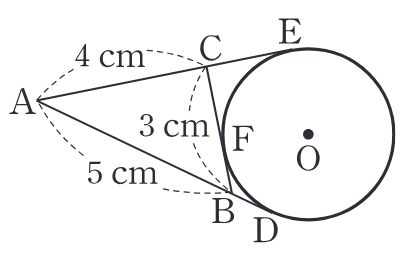
\includegraphics[width=\dmfigw]{figures/fig-0345.png}\end{minipage}\par
\begin{choicesii}{\rule[-3ex]{0pt}{8ex}$1\mkern3mu \mathrm{cm}$}{\rule[-3ex]{0pt}{8ex}$\dfrac{4}{3}\mkern3mu \mathrm{cm}$}{\rule[-3ex]{0pt}{8ex}$\dfrac{3}{2}\mkern3mu \mathrm{cm}$}{\rule[-3ex]{0pt}{8ex}$\dfrac{5}{3}\mkern3mu \mathrm{cm}$}{\rule[-3ex]{0pt}{8ex}$2\mkern3mu \mathrm{cm}$}\end{choicesii}
